\chapter{学生实验}

\section{验证玻意耳-马略特定律}

在这个实验中,我们用一个带有刻度的注射器近似地验证玻意耳-马略特定律.

实验研究的对象是封闭在注射器里的空气柱,空气柱的体积可由注射器上的刻度直接读出.空气柱的压强$p=p_0\pm \dfrac{F}{S}$,其中$p_0$为大气压强,$F$为活塞对空气柱的压力或拉力,$S$为活塞的横截面积.(考虑一下,哪种情况取正号,哪种情况取负号.)

实验时,先用弹簧秤称出活塞和框架的重量,用刻度尺测出注射器的全部刻度的长度,用这个长度去除它的容积即得活塞的横截面积$S$.记下气压计(全班共用一个)指示的大气压强$p_0$.

将活塞插入注射器内一部分后,将注射器的小孔堵住,以封入一定质量的空气.

把注射器固定好,在框架的两侧加挂钩码,使空气柱的体积减小(图9.1).改变钩码的个数,再做两次,记下每次加挂的钩码数和相应的空气柱的体积.
\begin{figure}[htbp]
    \centering
    \begin{minipage}[t]{0.48\textwidth}
        \centering
        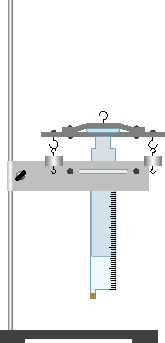
\includegraphics{fig/B/9-1.pdf}
        \caption{}\label{fig_B_9-1}
    \end{minipage}
    \begin{minipage}[t]{0.48\textwidth}
        \centering
        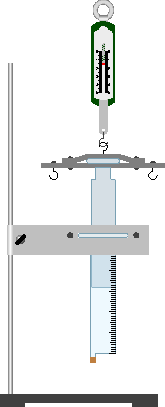
\includegraphics{fig/B/9-2.pdf}
        \caption{}\label{fig_B_9-2}
    \end{minipage}
\end{figure}

然后,用弹簧秤钩住活塞框架的上边,慢慢竖直提起活
塞,使空气柱的体积增大(图9.2),记下三组每提到一定高度时弹簧秤的读数和相应的空气柱的体积.

把记录的数据填入自己设计的表格里,根据公式$p=p_0\pm \dfrac{F}{S}$算出各个压强值(要注意活塞和框架的重量对压强的影响),求出各个压强$p$跟相应的体积$V$的乘积.比较这些乘积,能得出什么结论?

\section{验证气体状态方程}
这个实验,我们利用实验一的装置来验证气体状态方程.

跟实验一一样,先用弹簧秤称出活塞和框架的重量;测出注射器的全部刻度的长度,求出活塞的横截面积$S$;记下这时的大气压强$p_0$.在注射器内封入一定质量的空气.
\begin{figure}[htbp]
    \centering
    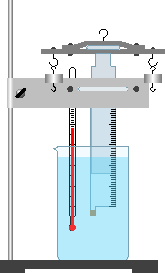
\includegraphics{fig/B/9-3.pdf}
    \caption{}\label{fig_B_9-3}
\end{figure}

照图9.3那样,固定好注射器和烧杯.在活塞框架的两侧加挂钩码,用公式$p=p_0+ \dfrac{F}{S}$计算出空气柱的压强(注意压力$F$中应包括活塞和框架的重
量).向烧杯里倒入适量的水,使注射器内的空气柱位于水面之下.经过两分钟左右,用温度计测出水的温度$t$,可以认为这个温度就是空气柱的温度,把它换算成热力学温度$T$.记下这时空气柱的体积$V$.

改变加挂的钩码数和烧杯中水的温度,再分别做四次上面的实验.

把上面得到的数据填入自己设计的表格里,并算出每次
实验得到的$pV/T$的值,看看它们是否相等,从实验可以得出什么结论?

\section{测定冰的熔解热}

单位质量的某种物质熔解成同温度的液体时吸收的热量,叫做这种物质的熔解热.在这个实验里我们利用量热器用混合法来测定冰的熔解热.

设有$m_{\text{冰}}$克的冰,温度为0$^\circ$C,与$m_{\text{水}}$克温度为$t_0$的水混合,冰全部熔解跟水混合以后的平衡温度为$t$.$m_{\text{冰}}$克冰熔解成水并升高到温度$t$吸收的热量,等于$m_{\text{水}}$克水以及盛水容器从温度$t_0$下降到温度$t$放出的热量,即
\[m_{\text{冰}}\lambda+m_{\text{冰}}c_{\text{水}}t=(m_{\text{水}}c_{\text{水}}+m_{\text{筒}}c_{\text{筒}})(t_0-t)  \]
其中,$\lambda$为冰的熔解热,$c_{\text{水}}$为水的比热,$c_{\text{筒}}$为容器的比热,$m_{\text{筒}}$为容器的质量,这样,把$c_{\text{水}}$和$c_{\text{筒}}$作为已知量,$m_{\text{冰}}$、$m_{\text{水}}$、$m_{\text{筒}}$和$t_0$、$t$都可以由实验获得,从而利用上式求出冰的熔解热$\lambda$.

实验开始时,先用天平称出量热器小筒的质量$m_{\text{筒}}$(包括搅拌器),然后把比室温高10—15$^\circ$C的温水(150克左右)倒入量热器小筒,再称出水和小筒的质量,算出水的质量$m_{\text{水}}$.把装着水的量热器小筒放在大筒的木架上,用温度计测出水和量热器小筒的初温$t_0$.把准备好的温度为0$^\circ$C的冰块\footnote{实验室里,冰水混合物的温度可以认为是0$^\circ$C.}(20克左右)迅速放入小筒的水中,并盖好量热器盖子,搅动小筒中的水,同时观察插入量热器里的温度计,当温度下降到最低
时,记录下来的温度$t$就是冰、水混合后的平衡温度,最后再称量一下量热器小筒和水的质量(其中包括冰的质量),算出冰的质量$m_{\text{冰}}$.

把由实验得到的数据代入第二段中的公式,求出冰的熔
解热,水的比热$c_{\text{水}}$,可取为$4.2\times10^3{\rm J}/({\rm kg}\cdot {}^\circ{\rm C})$,铝制小筒的比热$c_{\text{筒}}$可取为$8.9\times10^2 {\rm J}/({\rm kg}\cdot {}^\circ{\rm C})$,铜制小筒的比热$c_{\text{筒}}$可取为$3.9\times10^2{\rm J}/({\rm kg}\cdot {}^\circ{\rm C})$.

实验中要注意读准温度计的示数,冰块不宜太大,为什么?在这个实验中,误差的主要来源是什么?

\section{测定空气的相对湿度}
这个实验我们学习测定空气的相对湿度,实验装置如图9.4所示.圆柱形金属盒的一个底面十分光亮,侧面有开口,开口旁边有一小孔,用来插入温度计,环形金属片套在金属盒上,它的一面也是十分光亮,井与金属盒的光亮面在同一平面内,金属盒和环形片用胶木垫圈隔开,防止相互间的热传导,搅拌器插在开口中.
\begin{figure}[htbp]
    \centering
    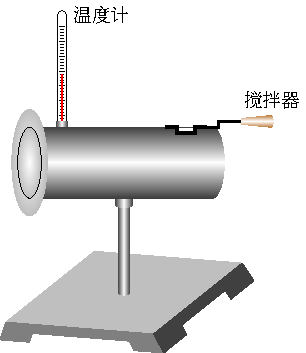
\includegraphics{fig/B/9-4.pdf}
    \caption{}\label{fig_B_9-4}
\end{figure}

实验时,先记录下实验室的温度,用柔软的绒布仔细地把金属盒和环形片的光亮面擦得十分干净,在金属盒里注入约
半盒室温的水,再向水里投入适量的碎冰块(注意不要沾污光亮面),装上温度计,并使它的刻度向着金属盒的光亮面,搅动冰块,使水温迅速下降,同时密切注视金属盒和环形片的光亮面,当金属盒的光亮面上刚刚出现细小的露滴时,记录下这一瞬间盒里水的温度,等水的温度又开始上升,金属盒光亮面
上的细小的露滴完全消失时,再记录下这一瞬间的温度,两次温度的平均值就是露点.

从课本里查出温度为测得的露点时水的饱和汽压$p$,这就是测量时空气中水蒸气的压强,即空气的绝对湿度,再查出测量时的室温下水的饱和汽压$P$.此时的相对湿度就是
\[B=\frac{p}{P}\times 100\%\]

\section{电场中等势线的描绘}
在这个实验里,我们学习用描迹法画出电场中平面上的等势线.

如图9.5所示,在平整的木板上铺一张白纸,白纸上依次铺放复写纸和导电纸,导电纸有导电物质的一面向上,白纸、复写纸和导电纸一起用图钉固定在木板上,导电纸上平放着跟它接触良好的两个圆柱形电极,电极A与电源的正极相连作为正电荷,电极$B$与电源的负极相连作为负电荷\footnote{我们在第六章学习的是静电场.直接接绘静电场中的等势线是相当困难的,由于静电场和稳恒电流场遵守的规律相似,这里是用在导电纸上形成的稳恒电流场模拟静电场来做实验.}.两电极之间的距离约为10厘米,电压约为6伏.
\begin{figure}[htbp]
    \centering
    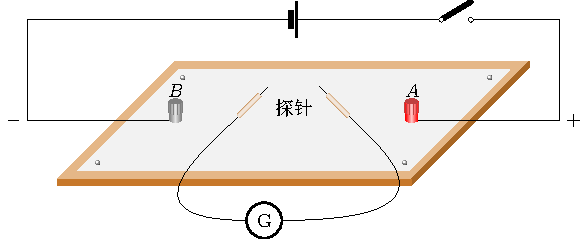
\includegraphics{fig/B/9-5.pdf}
    \caption{}\label{fig_B_9-5}
\end{figure}

现在,我们来描绘正、负电荷$A$、$B$在纸面上的等势线.从灵敏电流表的两个接线柱引出两个探针,用来探测导电纸上的等势点.先在导电纸平面两电极的连线上,选取间距大致相等的五个点作为基准点,并用探针把它们的位置复印在白纸上,在某一基准点将一个探针跟导电纸相接触,然后在导电纸平面上两电极连线的一侧,距此基准点约1厘米处再选一个点,在此点将另一探针跟导电纸相接触,一般这时会看
到电流表的指针有偏转,左右移动另一探针的位置,直到找到一点,使电流表的指针没有偏转为止,电流表的指针没有偏转,说明这个点跟基准点的电势相等,用探针把这个点的位置复印在白纸上,照上述方法,在这个基准点的两侧,各探测出五个等势点,每个等势点大约相距1厘米.用同样的方法,探测出另外四个基准点的等势点.最后,取出白纸.根据五组等势点画出五条平滑的曲线,它们就是等势线,你能不能根据这些等势线在白纸上画出两个异种电荷的电力线:画一画看.

\section{利用电容器放电测电容}
现在,我们通过实验来学习一种测量电容器电容的简单方法.

我们知道,电容器的电容等于电容器所带电量跟两极之
因此,如果测量出某一电压下间的电势差的比值,即$C=Q/U$.因此,如果测量出某一电压下
电容器所带的电量,就可以求出电容器的电容.怎样才能测量出电容器所带的电量呢?
\begin{figure}[htbp]
    \centering
    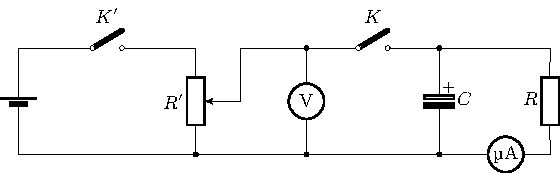
\includegraphics{fig/B/9-6.pdf}
    \caption{}\label{fig_B_9-6}
\end{figure}

测量电路如图9.6所示,合上电键$K'$、$K$,对电容器$C$充电.当电容器两端电压$U_c$上升到某一稳定电压$U$时,充电完毕.然后将电键$K$打开,这时容器通过电阻$R$放电,放电电流$i_c$随时间$t$的增加而逐渐减小,放电完毕时$i_c=0$.在电容器放电过程中,如果在某一时刻的放电电流为$i_c$,那么在一小段时间间隔$\Delta t$里,从电容器正极转移到负极上的电量就等于$i_c\Delta t$,将整个放电过程中每小段时间所转移的电量加起来,就得到电容器所带的电量$Q$.

按图9.6接好线路,电源可用学生电源,电容器$C$可选用
470微法的电解电容器,微安表可选用500微安量程的,$R$用27
千欧的定值电阻,接线时要注意电解电容器的极性不要接反.接通电源后,先合上电键$K$,调节变阻器$R'$使伏特表指示到实验需要的电压值12伏,然后合上电键$K$,给电容器充电,充电完毕,记下这时伏特表和微安表的读数.把电键$K$打开,同时开始计时,并且每间隔5秒钟读取一次微安表的电流值,直到电流值减至零为止.

根据记录的数据,在坐标纸上,以时间$t$为横坐标,以电流$i_c$为纵坐标作出$i_c$-$t$图象,然后再根据所画的$i_c$-$t$图象,求出电容器所带电量$Q$(同学们思考一下,怎样利用$i_c$-$t$图象求出电量$Q$),最后计算出电容器的电容.

\section{测定金属的电阻率}
这个实验是测定金属的电阻率.

电阻定律告诉我们,用电阻率为$\rho$制成的长$\ell{\rm m}$、横截面积$S{\rm m^2}$的导线的电阻
\[R=\rho\frac{\ell}{S}\]

因此,测出一段导线的长度和直径(由直径可以算出横截面积)以及这段导线的电阻,就可以求出制成这段导线的材料的电阻率.

现在有一段长约0.5米、直径约0.3毫米,阻值约3欧姆的金属导线,你应当选用哪些实验器材来测定它的电阻率?考虑一下,这个实验应当怎样进行?通过实验,你测得制成这段
导线的材料的电阻率是多少?

需要注意的是,在给导线通电时,电流不宜太大,想想看,这是为什么?

\section{把电流表改装为伏特表}
我们学习了把电流表改装为安培表和伏特表的原理,在这个实验里,我们练习把电流表改装为伏特表.

改装电流表,需要知道它的三个数据:满度电流$I_g$,满度电压$U_g$(电流表的指针偏转到满刻度时加在表头上的电压)和内电阻$r_g$.这三个数据中,知道任何两个,就可以根据欧姆定律算出第三个,电流表的$I_g$可以从刻度盘上直接读出,$r_g$可用实验方法测出,于是就可以算出$U_g$.
\begin{figure}[htbp]
    \centering
    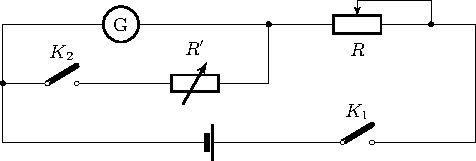
\includegraphics{fig/B/9-7.pdf}
    \caption{}\label{fig_B_9-7}
\end{figure}

我们利用图9.7所示的电路来测定电流表的内电阻$r_g$.$R$可用470千欧的电位器\footnote{电位器是一种可以连续调节电阻值的变阻器,常用作分压器.},$R'$是电阻箱,合上电键$K$,调整电位器$R$,使电流表指针偏转到满刻度(要注意,不应使通过电流表的电流超过它的满度电流值,以免把表烧坏),然后再合上电键$K_2$,调整电阻箱$R'$的阻值,使电流表指针偏转到正好是满刻度的一半,当$R$比$R'$大很多时,接入$R$后,干路中电流变化不大,因此可以认为$r_g=R'$.


测出$r_g$后,再计算出电流表的满度电压$U_g$,然后算出把它改装为2伏特的伏特表时,应该串联多大的电阻$R_1$.在电阻箱上取好阻值$R_1$,把电流表跟电阻箱串联起来,就是一个量程是2伏特的伏特表了.
\begin{figure}[htbp]
    \centering
    \begin{minipage}[t]{0.48\textwidth}
        \centering
        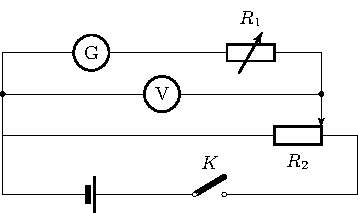
\includegraphics{fig/B/9-8.pdf}
        \caption{}\label{fig_B_9-8}
    \end{minipage}
    \begin{minipage}[t]{0.48\textwidth}
        \centering
        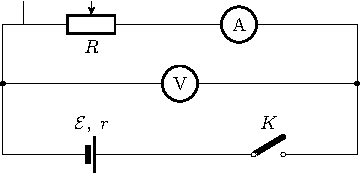
\includegraphics{fig/B/9-9.pdf}
        \caption{}\label{fig_B_9-9}
    \end{minipage}
\end{figure}
    

最后把改装成的伏特表跟标准伏特表核对一遍.实验电路如图9.8所示,$V$是标准伏特表,改变变阻器$R_2$的触点,使$V$的读数分别为0.5伏特、1伏特、1.5伏特、2伏特时,核对一下改装的伏特表的读数是否正确,核对时要注意搞清楚改装后电流表上刻度的每一小格表示多大电压.最后算出改装的伏特表满刻度时的百分误差.例如改装的伏特表在满刻度2伏特时,标准伏特表的读数为2.1伏特,那么满刻度时的百分误差就是
\[\frac{|2.1-2|}{2.1}=4.8\%\]

\section{用安培表和伏特表测定电池的电动势和内电阻}

这个实验是用安培表和伏特表测出电流和路端电压,再用闭合电路的欧姆定律来求出电动势和内电阻,实验电路如图9.9所示.

我们知道,只要改变$R$的阻值,测出两组$I$、$U$的数据.代入方程组
\[\begin{split}
    \mathcal{E}&=U_1+I_1r\\
    \mathcal{E}&=U_2+I_2r\\
\end{split}\]
就可以求出电动势$\mathcal{E}$和内电阻$r$,这样做在原理上虽然很简单,但偶然误差却很大.

为了减小偶然误差,我们可以多测出几组$I$、$U$的数据,求出几组$\mathcal{E}$、$r$值,最后分别算出它们的平均值.此外,物理实验中还经常用作图法,现在我们就来学习作图法.

利用变阻器$R$测出几组$I$、$U$值后,在坐标纸上以$I$为横坐标,$U$为纵坐标,画出$U$-$I$关系图象,根据闭合电路的欧姆定律,$U=\mathcal{E}-Ir$,因此$U$是$I$的一次函数,它们的图象应该是一条直线,你得出的是不是一条直线?把这条直线延长,使
它跟纵轴相交,这个交点有什么物理意义?在图象中内电阻是怎样表示出来的?你怎样利用自己作出的图象来得到电池的电动势和内电阻?

这里还要作一点说明,作图时要适当选取横坐标、纵坐标的比例和坐标的起点,使实验数据大致布满整个图纸,不要集中在一边或一角.这个实验的$U$值不宜过小,因此纵坐标$U$的起点不要从零开始,而横坐标$I$仍要以零为起点.(为什么?)

\section{练习使用万用电表}
万用电表(常简称为万用表)是一种多用仪表,一般可以用来测量电流、电压、电阻等,并且每一种测量项目有几个量
程,由于万用表具有用途多、量程广、使用方便等优点,因此得到了广泛的应用,这个实验我们来学习万用表的使用.

万用表的型号很多,但使用方法基本相同,下面以J0411型万用表为例来说明它的使用方法和注意事项.
\begin{figure}[htbp]
    \centering
    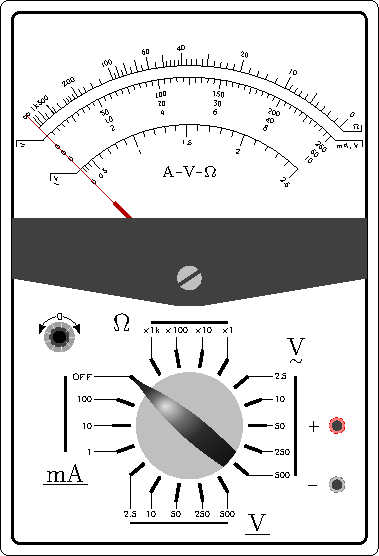
\includegraphics{fig/B/9-10.pdf}
    \caption{}\label{fig_B_9-10}
\end{figure}

J0411型万用表的外形如图9.10所示.它的上半部是表
头,表盘上有电阻、电流、电压等各种量程的刻度,有的刻度是均匀的,因此合用一个刻度.下半部是选择开关,它的四周刻着各种测量项目和量程.应当注意,电流和电压又分为直流(用符号“$-$”表示)和交流(用符号“$\sim$”表示),要区别开,不要弄错.另外还有欧姆档的调零旋钮和测试笔插孔.

测量前,应先检查表针是否停在左端的“0”位置,否则,要用小螺丝刀轻轻地转动表盘下边中间的调整定位螺丝,使指针指零.万用表有两根测试笔,将红表笔和黑表笔分别插入正($+$)、负($-$)测试笔插孔.

测量时,应把选择开关旋到相应的项目和量程上,读数时,要看跟选择开关的档位相应的刻度.

测量电流时,跟电流表一样,应把万用表串联在被测电路里;对于直流电,还必须使电流从红表笔流进万用表,从黑表笔流出来.

测量电压时,跟电压表一样,应把万用表和被测部分并联;对于直流电,必须用红表笔接电势较高的点,用黑表笔接电势较低的点.

测量电阻时,在选择好选择开关的档位后,要先把两根表笔相接触,调整欧姆档的调零旋钮,使指针指在电阻刻度的零位上(注意,电阻刻度的零位在表盘的右端),然后再把两表笔分别与待测电阻的两端相接,进行测量.换用欧姆档的另一量程时,需要重新调整欧姆档的调零旋钮,才能进行测量.应当注意,测量电阻时待测电阻要跟别的元件和电源断开.(为什么?)

测量时,注意手不要碰到表笔的金属触针,以保证安全和测量的准确;使用后,要把表笔从测试笔插孔拔出,井且不要把选择开关置于欧姆档,以防电池漏电;长期不使用时,应把电池取出.

在了解了你使用的万用表之后,就可以按照老师的要求,
来进行电流、电压和电阻的测量了.

\section{用惠斯通电桥测电阻}

这个实验是用滑线式电桥来测电阻.
\begin{figure}[htbp]
    \centering
    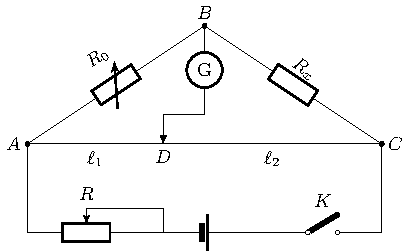
\includegraphics{fig/B/9-11.pdf}
    \caption{}\label{fig_B_9-11}
\end{figure}

实验电路如图9.11所示,其中$R_x$是待测电阻,$R_0$是作已知电阻用的电阻箱,$G$是灵敏电流表,按图接好电路后,先把变阻器$R$调到阻值较大的位置,然后进行实验.

根据误差理论,触头$D$在$AC$中点附近电桥平衡时实验误
差较小(这个道理在这里就不讲了),我们先用万用表测出$R_x$的大约值,在电阻箱上选取跟它接近的某一阻值$R_0$.合上电键$K$,把滑动触头$D$移到电阻线$AC$中点附近業一位置,瞬时按下触头,一般会看到电流表的指针有偏转,稍稍移动触头,再把它瞬时按下,比较电流表指针两次偏转的情况.根据指针偏转的方向是否相同和偏角是增大还是减小,你应该能判断出应向哪个方向移动触头才能使电桥平衡.继续移动触头直到电桥平衡,电流表的指针不再偏转为止.要注意,每次按下触头的时间要尽量短,用力不要过大,更不要在按下触头后又设法移动它.

电桥平衡后,打开电键$K$,读出或量出$AD$的长度$\ell_1$和$DC$的长度$\ell_2$,根据$R_0/R_x=\ell_1/\ell_2$求出$R_x$,这就初步测出了$R_x$的值.

现在来进一步更精确地测定$R_x$.先在电阻箱上取跟初步测出的$R_x$相近的阻值,重新使电桥平衡,然后逐步减少变阻器$R$的阻值,以增大$AC$间的电压,但要注意通过电阻线$AC$
的电流不能超过它的允许值,可以看到,每当$R$的阻值减少后,按下触头$D$时电桥又可能不平衡了,每次都要重新调整触头$D$的位置,才能使电桥恢复平衡.同学们想想看,这是什么道理.要注意这时每次都只能微调触头$D$的位置,以免烧毁电流表,当$R$的阻值减小到一定程度时,使电桥平衡,然后读出或量出$l_1$和$l_2$,利用公式算出$R_x$.为什么现在求出的$R_x$比初测的$R_x$精确?

\section{测定铜的电化当量}
在这个实验里,我们根据法拉第电解第一定律$m=kIt$,测出$m$、$I$和$t$的值,从而确定电化当量$k$.
\begin{figure}[htbp]
    \centering
    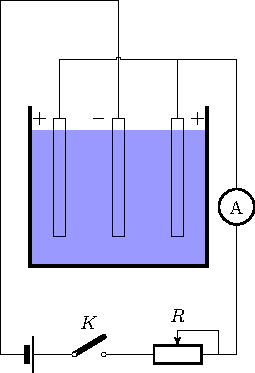
\includegraphics{fig/B/9-12.pdf}
    \caption{}\label{fig_B_9-12}
\end{figure}

准备三块铜片,两块作为阳极,一块作为阴极,并用细砂纸把铜片擦干净,用天平仔细称量作为阴极的铜片的质量.把铜片放入盛有硫酸铜溶液的电解槽内,按照图9.12接好电路(注意电源和安培表的正负端不要接错),合上电键$K$,调节变阻器$R$使安培表的读数为2安培左右,并开始计时.25—30分钟后,打开电键$K$,停止电解.注意要在整个电解过程中,调节变阻器使电流强度保持不变.电解结束后,取出电极,用酒精灯把阴极板烘干,再用天平仔细称量出这时阴极板的质量,比较两次称量的阴极板的质量,就可以得到电解过程中在阴极板上析出的铜的质量$m$.把$m$、$I$和$t$带入法拉第电解第一定律公式,算出铜的电化当量.

你测定的铜的电化当量是多少?跟课本上给出的数值相差多少?考虑一下,实验误差的主要原因是什么?应当怎样改进这个实验?

\section{练习使用示波器}
示波器是一种常用的电子仪器,它的核心部分是一只示波管,利用它能够直接观察电信号随时间而变化的情况,并且可以测量电压和电流.我们现在初步学习一下示波器的使用方法,在后面的实验里还要多次用到它.

示次器的型号很多,使用方法基本相同,下面以J2459型示波器(图9.13)为例来说明.
\begin{figure}[htbp]
    \centering
    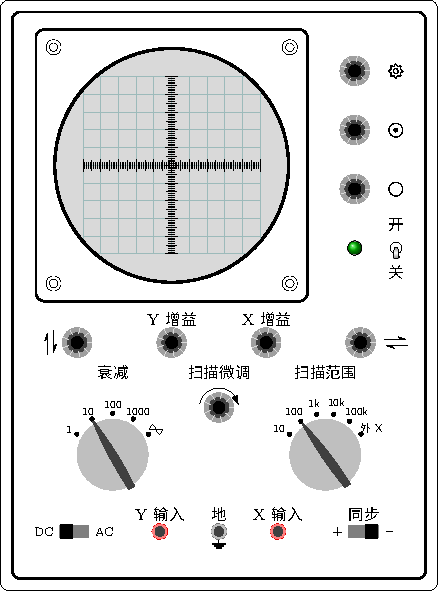
\includegraphics{fig/B/9-13.pdf}
    \caption{J2459型示波器的面板}\label{fig_B_9-13}
\end{figure}

我们先来了解示波器面板上各个旋纽和开关的名称和作用.荧光屏右边最上端的旋钮是辉度调节“$\star$”,用来调节图象的亮度,顺时针旋转时亮度逐渐增大,它下面的旋钮是聚焦调节“$\odot$”和辅助聚焦“$\textcircled{~}$”,这两个旋钮配合着使用,能使电子射线会聚,在荧光屏上产生一个小的亮斑,得到清晰的图象,再下面是电源开关和指示灯,用后盖板上的电源插座接通电源后,把开关板向“开”的位置,指示灯亮,经过一两分钟
的预热,示波器就可以使用了.

荧光屏下边第一行左右两端的旋钮是竖直位移“$\uparrow\downarrow$”和水平位移“$\leftrightarrows$”,分别用来调整图象在竖直方向和水平方向的位置.它们中间的两个旋钮是“Y增益”和“X增益”,分别用来调整图象在竖直方向和水平方向的幅度,顺时针旋转时,幅
度连续增大.

中间一行左边的大旋钮是“衰减”,它有1, 10、100、1000四档,最左边的“1”档不衰减,其余各档分别使输入电压衰减为
原来的1/10、1/100、1/1000,因此图象在竖直方向的幅度都减小为前
一档的十分之一;最右边的正弦符号“\tikz \draw[x=.7ex,y=1ex] (0,0) sin (1,1) cos (2,0) sin (3,-1) cos (4,0)--(0,0);”档不是衰减,而是由
示波器内部自行提供竖直方向的交流试验信号电压,可用来观察正弦波形或检查示波器是否正常工作.右边的大旋钮是“扫描范围”,也有四档,可以改变加在水平方向的扫描电压的频率范围,左边第一档是10—100赫兹,向右旋转每升高一档,扫描频率都增大10倍,最右边的是“外X”档,使用这一档时,机内没有加扫描电压,水平方向的电压可以从外部输入.中间的小旋钮是“扫描微调”,用来调整水平方向的扫描频率,顺时针转动时频率连续增加.

底下一行中间的旋钮“Y输入”、“X输入”和“地”分别是竖直方向、水平方向和公共接地的输入接线柱.左边的“DC、AC”是竖直方向输入信号的直流、交流选择开关,置于“DC”位置时,所加的信号电压是直接输入的;置于“AC”位置时,所加的信号电压是通过一个电容器输入的,它可以让交流信号通过而隔断直流成分,右边的“同步”也是一个选择开关,置于“$+$”位置时,扫描由被测信号正半周起同步,置于“$-$”位置时,扫描由负半周起同步.

现在,我们来练习使用示波器.先把辉度调节旋钮反时针转到底,竖直位移和水平位移旋钮旋转到中间位置,衰减旋钮置于最高档,扫描范围旋钮置于“外X”档,打开电源开关,
指示灯亮,经预热后,顺时针旋转辉度调节旋钮,屏上即出现一个亮斑,亮斑的亮度要适中,注意不应使亮斑过亮,特别
是当亮斑长时间停留在屏上不动时,应把亮度减弱,以免损伤荧光屏,减少示波管的使用寿命,旋转聚焦调节和辅助聚焦旋钮,观察亮斑的变化,使亮斑最圆最小,旋转竖直位移旋钮,观察亮斑的上下移动,旋转水平位移旋钮,观察亮斑的左右移动.

把X增益旋钮顺时针转到三分之一处,扫描微调旋钮反时针转到底,扫描范围旋钮置于最低档.可以看到扫描的情形:亮斑从左向右移动,到右端后又很快回到左端,顺时针旋转扫描微调以增大扫描频率,可以看到亮斑迅速移动成为一条亮线,调整X增益,可以看到亮线长度的改变.

现在给竖直方向加一个直流电压.事先把扫描范围旋钮置于“外X”档,使亮斑位于屏的中心,把“DC、AC”开关置于“DC”位置,照图9.14连接电路,直流电源用一、二节干电池即可,逐步减小衰减档,观察亮斑的向上偏移,再调整Y增益使亮斑偏移一段适当的距离,调整变阻器改变输入电压,可以看到亮斑的偏移随着改变,电压越高,偏移越大,调换电池的正负极,改变输入电压的方向,可以看到亮斑改为向下偏移.
\begin{figure}[htbp]
    \centering
    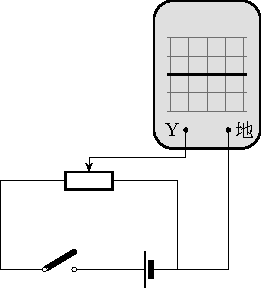
\includegraphics{fig/B/9-14.pdf}
    \caption{}\label{fig_B_9-14}
\end{figure}

亮斑偏移的距离跟输入的电压成正比,因而利用示波器
能够测量电压,J2459型示波器的竖直位移已经校准,当衰减旋钮处在“1”的位置,Y增益旋钮顺时针转到底时,如果输入电压为50毫伏,则亮斑恰好偏移1格.这样,我们就可以根据亮斑偏移的格数来算出输入的电压值,测量时要注意把Y增益旋钮顺时针转到底;衰减旋钮处在10、100或1000档时,算出的电压值应乘以相应的倍数,现在来测一节干电池的电压,你测出的数值是多少?

利用示波器还可以测量电流.把一个已知阻值的小电阻串联在待测电流的电路里(或利用原电路中的已知电阻),用示波器测量这个电阻两端的电压,利用欧姆定律就可以算出电路中的电流.这种测量我们就不做了.

实验完了,关机前要注意把辉度调节旋钮反时针方向转到底,使亮度减到最小.

